\documentclass[aspectratio=169]{beamer}
\usetheme{default}
\usecolortheme{rose}
\usepackage{graphicx}
\setbeamertemplate{caption}[numbered]
\graphicspath{{../figures/}}
\usepackage{subcaption}



\title{p5607 acoustic analysis -- preliminary}
%\author{Clay Wood}
%\date{06 May 2020}



\begin{document}
	
	
\begin{frame}[plain]
    \maketitle
\end{frame}


\begin{frame}{}

	\begin{figure}
		\centering
		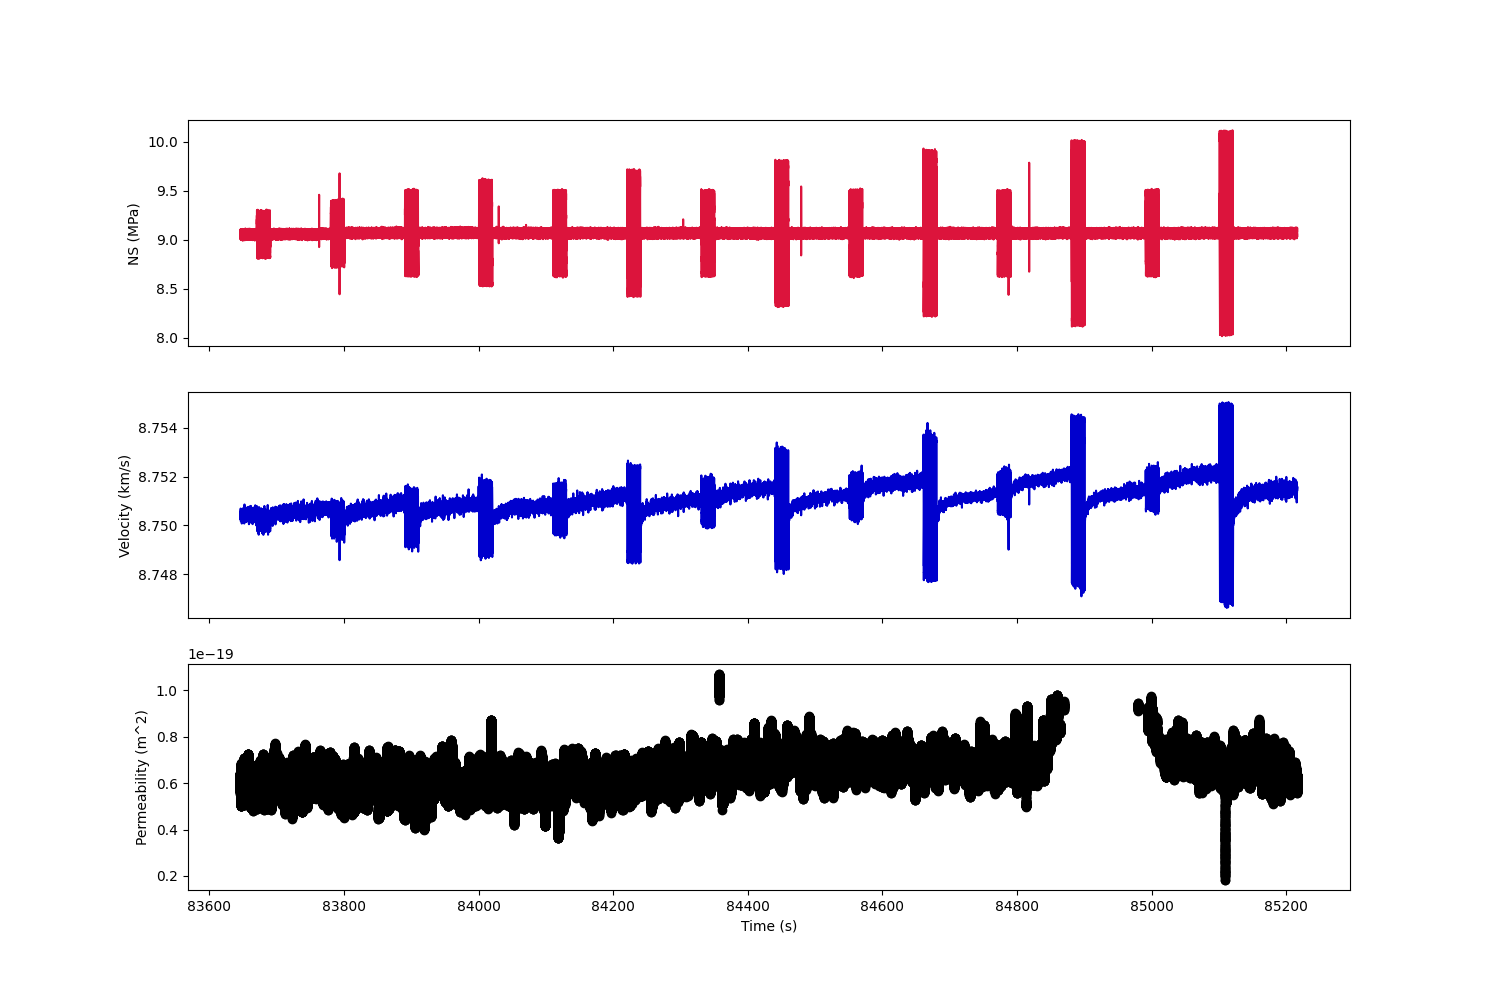
\includegraphics[height=8cm]{../rel_chg_analysis/p5607_run1_prelim_tr5.png}
	\end{figure}

\end{frame}

\begin{frame}{}

	\begin{figure}
		\centering
		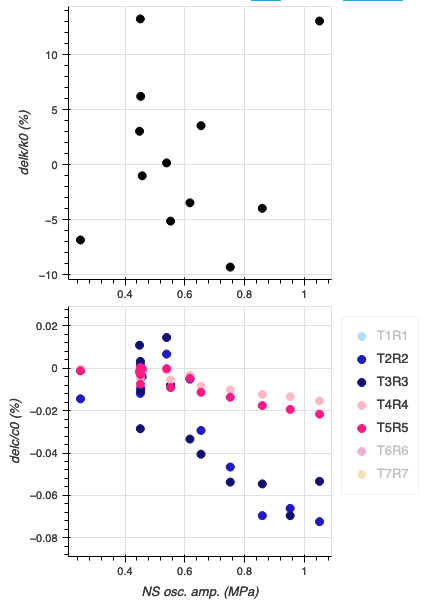
\includegraphics[height=6cm]{../rel_chg_analysis/p5607_run1_prelim_delc_NS.png}
	\end{figure}

\end{frame}


\begin{frame}{}
	
	\begin{alertblock}{To-do:}
		\begin{itemize}
			\item fix x-corr windows for following pairs: TR1, TR6, TR7
			\item update velocity function with new sideblock geometry
		\end{itemize}
	\end{alertblock}
	

\end{frame}



\end{document}
